% Provenance (never printed): see sources/outline_sources.md (Year 2: energy geology --- the
% petroleum system quantified, unconventional resources, geothermal systems, uranium deposits,
% geological storage of carbon dioxide).
% Kerogen kinetics and elemental analyses: Fletcher and Pugmire (DOE, OSTI 1176871); kerogen
% types and Easy%Ro: Advanced Chemistry Basins Project (DOE, OSTI 830009); maturity thresholds:
% USGS MF-2008-B; TTI: Waples (1980) and Hammerschmidt et al. (2014); volumetrics and CO2
% storage: DOE/NETL (2008) and IPCC SRCCS (2005) chapter 5; geothermal: USGS OFR 2008-1296 and
% FS 2008-3082; uranium: USGS Bulletin 1693; Oklo: OSTI abstract records. Ledger rows in
% sources/ledger/book4.md; curves from figdata/bachelor-2/maturation.py and co2_density.py,
% numbers from the Book 4 second-writer scratch calculator calc/ch30.py.
% Geology and sourced numbers only: no advocacy, no policy.
\chapter{Geologi Energi}\label{ch:b2:energy-geology}

Minyak bumi adalah sisa organisme mikroskopis yang terkubur bersama lumpur lalu dimasak selama jutaan tahun pada
sekitar \qty{100}{\celsius}; energi panas bumi adalah kehangatan Bumi yang sama, yang diambil secara langsung.
Keduanya dikendalikan oleh suhu dan waktu: yang pertama oleh laju suatu reaksi kimia ketika
batuan yang terkubur perlahan-lahan menghangat, yang kedua oleh banyaknya panas yang disimpan suatu volume batuan dan seberapa cepat air
dapat membawanya ke sumur. Bab ini mengkuantifikasi sistem petroleum, lalu beralih ke sumber daya yang
tidak memiliki salah satu unsurnya, ke panas bumi dan ke uranium, dan diakhiri dengan operasi kebalikannya:
mengembalikan karbon dioksida ke bawah tanah.
% ledger: earle:oil-window, earle:organic-preservation

\begin{recall}
\textbf{Dari volume-volume sekolah}: batuan sumber, kerogen, pematangan, jendela minyak, migrasi,
batuan reservoir, batuan penutup, perangkap, batuan penimbun, dan sistem petroleum; batu bara dan peringkat batu bara; energi panas bumi.
\textbf{Dari volume Tahun 1}: aliran panas dan geoterm; porositas dan permeabilitas; tekanan fluida
pori, tegangan efektif, dan kriteria Coulomb; log lubang bor; cekungan sedimen dan
penurunan cekungan. \textbf{Dari buku-buku kimia}: hukum Arrhenius, energi aktivasi, reaksi
orde pertama. \textbf{Dari buku-buku fisika}: peluruhan radioaktif, konstanta peluruhan, waktu paruh; titik
kritis suatu fluida. \textbf{Dari \cref{ch:b2:basins-compared}}: \omterm{def:b2:basins-compared:curve}{kurva penurunan}.
\textbf{Dari \cref{ch:b2:ore-deposits}}: \omterm{def:b2:ore-deposits:types}{tipe endapan bijih}, \omterm{def:b2:ore-deposits:grade}{tonase}.
\end{recall}

\section{Sistem petroleum secara kuantitatif}\label{sec:b2:energy-geology:petroleum}

Suatu sistem petroleum memerlukan batuan sumber yang kaya kerogen, reservoir, batuan penutup, perangkap, dan batuan penimbun
yang cukup tebal untuk memanaskan batuan sumber, dan peristiwa-peristiwanya harus terjadi dalam urutan yang benar: perangkap harus
sudah ada ketika minyak bermigrasi. Mengkuantifikasinya berarti menjawab tiga pertanyaan: jenis kerogen apa
yang dikandung batuan sumber, sejauh mana kerogen itu telah terkonversi, dan berapa banyak hasilnya yang berada di dalam
perangkap.
% ledger: magoon00:tps

\begin{definition}[Tipe kerogen, diagram van Krevelen]\label{def:b2:energy-geology:kerogen}
Yang disebut \emph{tipe kerogen}\index{tipe kerogen} adalah ketiga golongan kerogen menurut komposisi unsurnya:
tipe~I, sapropelik, yang paling kaya hidrogen, yang terutama menghasilkan minyak; tipe~III, humik atau bersifat batu bara,
miskin hidrogen, yang terutama menghasilkan metana; dan tipe~II, peralihan, sumber minyak sekaligus
gas. Yang disebut \emph{diagram van Krevelen}\index{diagram van Krevelen} adalah grafik rasio atom H/C
suatu kerogen terhadap rasio atom O/C-nya; tipe-tipe itu menempati wilayah yang berbeda di dalamnya, dan pematangan
menggeser kerogen ke arah H/C rendah dan O/C rendah.
\end{definition}

Tujuh kerogen belum matang yang tipenya diketahui, yang dianalisis dalam satu kajian laboratorium, memiliki H/C atom
1.51 dan 1.61 (tipe~I, di antaranya serpih minyak Green River di Utah, yang diendapkan di danau dan kaya akan
sisa alga), 1.22 sampai 1.28 (tipe~II, di antaranya Kimmeridge Clay di Laut Utara),
1.13 (tipe campuran~II/III), dan 0.99 (tipe~III, batu bara Cameo di Colorado). Kerogen Green
River, dengan \qty{77}{\percent} karbon menurut massa, rata-rata berkomposisi C$_{100}$H$_{150}$N$_3$O$_8$S: H/C 1.50 dan
O/C 0.08. Bila dipanaskan di laboratorium dengan laju \qty{10}{K} per menit, kerogen itu meninggalkan residu yang H/C-nya turun menjadi
1.20 pada \qty{460}{\celsius} dan 0.54 pada \qty{525}{\celsius}, sementara O/C-nya turun dari 0.08 menjadi sekitar
0.01: lintasan yang digambar di sisi kiri gambar di bawah.
% ledger: acb04:kerogens, fp14:gr-kerogen, fp14:gr-chars, mf88:thresholds
% values: GR3.9 kerogen H/C 1.486, O/C 0.080; chars 460 C 1.200/0.016, 525 C 0.544/0.011 (figdata maturation.py vk)

\begin{omfigure}
\centering
\begin{minipage}[b]{0.49\linewidth}\centering
\begin{tikzpicture}
\begin{axis}[omrecord, width=0.95\linewidth, height=5.0cm, xmin=0, xmax=0.12, ymin=0, ymax=1.8,
  xlabel={rasio atom O/C}, ylabel={rasio atom H/C}, xtick={0,0.04,0.08}, scaled x ticks=false,
  xticklabel style={/pgf/number format/fixed}, tick label style={font=\scriptsize},
  label style={font=\small}]
% computed in figdata/bachelor-2/maturation.py part vk; ledger: fp14:gr-kerogen, fp14:gr-chars
\addplot[omThm, line width=0.9pt, mark=*, mark size=1.3pt, -{Stealth[length=4pt]}] table[x=oc, y=hc] {figdata/out/bachelor-2-maturation-vk.dat};
\node[font=\scriptsize, text=omThm, anchor=north east] at (axis cs:0.081,1.45) {kerogen};
\node[font=\scriptsize, text=omThm, anchor=west] at (axis cs:0.013,0.52) {\qty{525}{\celsius}};
% ledger: acb04:kerogens (H/C of immature kerogens; O/C not reported)
\draw[omThm, line width=1pt] (axis cs:0.104,1.51) -- (axis cs:0.12,1.51);
\draw[omThm, line width=1pt] (axis cs:0.104,1.61) -- (axis cs:0.12,1.61);
\draw[omProp, line width=1pt] (axis cs:0.104,1.22) -- (axis cs:0.12,1.22);
\draw[omProp, line width=1pt] (axis cs:0.104,1.25) -- (axis cs:0.12,1.25);
\draw[omProp, line width=1pt] (axis cs:0.104,1.28) -- (axis cs:0.12,1.28);
\draw[omExo, line width=1pt] (axis cs:0.104,1.13) -- (axis cs:0.12,1.13);
\draw[omDef, line width=1pt] (axis cs:0.104,0.99) -- (axis cs:0.12,0.99);
\node[font=\scriptsize, text=omThm, anchor=east] at (axis cs:0.103,1.58) {I};
\node[font=\scriptsize, text=omProp, anchor=east] at (axis cs:0.103,1.25) {II};
\node[font=\scriptsize, text=omDef, anchor=east] at (axis cs:0.103,0.97) {III};
\end{axis}
\end{tikzpicture}
\end{minipage}\hfill
\begin{minipage}[b]{0.49\linewidth}\centering
\begin{tikzpicture}
\begin{axis}[omrecord, width=0.95\linewidth, height=5.0cm, xmin=60, xmax=220, ymin=0, ymax=1,
  xlabel={suhu (\unit{\celsius})}, ylabel={rasio transformasi},
  tick label style={font=\scriptsize}, label style={font=\small}]
% computed in figdata/bachelor-2/maturation.py part tr; ledger: fp14:gr-daem
\addplot[black!40, densely dotted] coordinates {(60,0.5) (220,0.5)};
\addplot[omDef, line width=1.1pt] table[x=t_c, y=tr1] {figdata/out/bachelor-2-maturation-tr.dat};
\addplot[omThm, line width=1.1pt] table[x=t_c, y=tr10] {figdata/out/bachelor-2-maturation-tr.dat};
\addplot[omDef, line width=0.6pt, densely dashed] table[x=t_c, y=app1] {figdata/out/bachelor-2-maturation-tr.dat};
\addplot[omThm, line width=0.6pt, densely dashed] table[x=t_c, y=app10] {figdata/out/bachelor-2-maturation-tr.dat};
\node[font=\scriptsize, text=omDef, anchor=east] at (axis cs:125,0.80) {\qty{1}{\celsius\per\Ma}};
\node[font=\scriptsize, text=omThm, anchor=west] at (axis cs:160,0.30) {\qty{10}{\celsius\per\Ma}};
\end{axis}
\end{tikzpicture}
\end{minipage}
\par\smallskip{\small Kiri: suatu \omterm{def:b2:energy-geology:kerogen}{diagram van Krevelen}. Lintasan merah adalah kerogen tipe~I Green River
dan residu-residunya setelah pemanasan laboratorium dengan laju \qty{10}{K} per menit sampai 400--\qty{525}{\celsius};
tanda-tanda di sisi kanan menunjukkan H/C tujuh kerogen belum matang bertipe~I (merah), II (jingga),
II/III (abu-abu), dan III (biru), yang O/C-nya tidak dilaporkan. Data: Fletcher dan Pugmire (2014);
Advanced Chemistry Basins Project (2004). Kanan: rasio transformasi kerogen Green River
yang dipanaskan dengan laju tetap sejak \qty{10}{\celsius}, dengan distribusi energi aktivasinya
(garis utuh) dan dengan energi rata-ratanya saja, menurut \eqref{eq:b2:energy-geology:maturation} (garis putus-putus).}
\end{omfigure}

Konversi kerogen menjadi petroleum adalah sekumpulan reaksi orde pertama, yang masing-masing mematuhi hukum
Arrhenius. Di dalam cekungan yang mengalami penurunan, suhu batuan sumber naik secara perlahan dan hampir
dengan laju tetap, sehingga hasil berikut menjadi inti model-model pematangan.

\begin{proposition}[Reaksi orde pertama pada laju pemanasan tetap]\label{prop:b2:energy-geology:maturation}
Misalkan suatu reaksi orde pertama dengan konstanta laju $k = A\,e^{-E/RT}$ berlangsung dalam bahan yang dipanaskan dengan
laju tetap $\beta = \mathrm{d}T/\mathrm{d}t$ sejak suhu $T_0$ yang membuat $k$ dapat diabaikan.
Fraksi yang belum terkonversi pada suhu $T$ adalah
\begin{equation}
x(T) = \exp\Bigl[-\frac{A}{\beta}\int_{T_0}^{T} e^{-E/RT'}\,\mathrm{d}T'\Bigr]
\approx \exp\Bigl[-\frac{A R T^2}{\beta E}\,e^{-E/RT}\Bigr] ,
\label{eq:b2:energy-geology:maturation}
\end{equation}
dengan pendekatan itu berlaku bila $E/RT \gg 1$; rasio transformasinya adalah $1 - x$.
\end{proposition}

\begin{proof}
Orde pertama berarti $\mathrm{d}x/\mathrm{d}t = -k x$. Dengan $\mathrm{d}t = \mathrm{d}T/\beta$,
$\mathrm{d}\ln x = -(A/\beta)\,e^{-E/RT}\,\mathrm{d}T$, dan integrasi dari $x = 1$ pada $T_0$ memberikan
bentuk pertama. Untuk integralnya, $\frac{\mathrm{d}}{\mathrm{d}T}\bigl[\frac{RT^2}{E}e^{-E/RT}\bigr]
= \bigl(1 + \frac{2RT}{E}\bigr)e^{-E/RT}$, sehingga integral itu sama dengan $\frac{RT^2}{E}e^{-E/RT}$ sampai
koreksi relatif berorde $2RT/E$, dan batas bawahnya tidak menyumbang apa pun karena $e^{-E/RT_0} \ll
e^{-E/RT}$.
\end{proof}

Ada dua akibat. Konversi terjadi dalam rentang suhu yang sempit, karena
$e^{-E/RT}$ berubah begitu cepat (latihan~\ref{exo:b2:energy-geology:11}). Dan pemanasan yang lebih lambat mengonversi
pada suhu yang lebih rendah: dengan $x = 1/2$, laju pemanasan yang sepuluh kali lebih cepat menaikkan suhu
konversi separuh sekitar $(RT^2/E)\ln 10$. Kinetika kerogen Green River, yang dicocokkan dengan
pirolisis laboratorium, adalah $A = \qty{9.21e13}{s^{-1}}$ dan $E/R = \qty{26800}{K}$ ($E =
\qty{223}{kJ/mol}$); dengan energi tunggal ini, konversi separuh terjadi pada \qty{136.4}{\celsius} untuk
\qty{1}{\celsius\per\Ma} dan pada \qty{150.9}{\celsius} untuk \qty{10}{\celsius\per\Ma}, pergeseran
\qty{14.5}{\celsius} dibandingkan dengan $6.26 \times \ln 10 = \qty{14.4}{K}$ yang diramalkan. Bila dipanaskan dengan laju
\qty{10}{K} per menit, kerogen yang sama terkonversi di dekat \qty{450}{\celsius}
(latihan~\ref{exo:b2:energy-geology:6}): waktu menggantikan suhu, itulah sebabnya kinetika
diukur dengan pirolisis pada sekitar 250 sampai \qty{600}{\celsius}, dan mengapa mengekstrapolasinya melintasi dua belas
orde besaran laju pemanasan membuat kedalaman jendela minyak yang diramalkan menjadi tidak pasti.
% ledger: fp14:gr-daem, acb04:kinetic-spread, codata:R
% values: Thalf 136.403 / 150.873 C; RT2/E 6.2587 K; lab 445.9 C (figdata maturation.py numbers, calc/ch30.py)

Kerogen yang sebenarnya memiliki ikatan dengan berbagai kekuatan, sehingga kinetikanya berupa distribusi energi
aktivasi, yang setiap fraksinya mematuhi proposisi itu; untuk kerogen Green River distribusinya
normal, dengan simpangan baku $\sigma/R = \qty{481}{K}$. Distribusi itu menyebarkan
konversi, seperti diperlihatkan sisi kanan gambar: pada \qty{150}{\celsius} kerogen yang dipanaskan dengan laju
\qty{1}{\celsius\per\Ma} telah \qty{93}{\percent} terkonversi, sedangkan yang dipanaskan sepuluh kali lebih cepat baru
\qty{48}{\percent}.
% ledger: fp14:gr-daem
% values: TR 0.927 / 0.484 at 150 C (figdata maturation.py numbers)

\begin{definition}[Reflektansi vitrinit, indeks waktu--suhu]\label{def:b2:energy-geology:maturity}
Yang disebut \emph{reflektansi vitrinit}\index{reflektansi vitrinit}, $R_o$, adalah persentase cahaya
datang yang dipantulkan oleh butir-butir vitrinit yang dipoles, suatu komponen organik batu bara dan kerogen,
yang diukur di bawah mikroskop; nilainya naik secara tak terbalikkan dengan pemanasan dan merekam kematangan termal tertinggi yang pernah dicapai suatu batuan. Yang disebut
\emph{indeks waktu--suhu}\index{indeks waktu--suhu} (TTI) Lopatin adalah jumlah
$\sum_n \Delta t_n\,2^n$ atas selang-selang \qty{10}{\celsius} yang telah dilalui suatu batuan,
dengan $\Delta t_n$ waktu dalam juta tahun yang dilewatkan dalam selang bernomor $n$, dengan $n = 0$
untuk 100 sampai \qty{110}{\celsius}, $n = 1$ untuk 110 sampai \qty{120}{\celsius}, $n = -1$ untuk 90 sampai
\qty{100}{\celsius}, dan seterusnya.
\end{definition}

Pada skala reflektansi, pembentukan minyak dari kerogen tipe~I dan II dimulai di dekat $R_o =
\qty{0.60}{\percent}$; di atas 1.20 sampai \qty{1.30}{\percent} minyak tidak stabil dan terurai menjadi
metana; tipe~III mulai menghasilkan metana di dekat \qty{0.73}{\percent}, dan pembentukan gas berlanjut sampai
sekitar \qty{4.8}{\percent}. Model-model menghitung $R_o$ seperti menghitung kerogen: model Easy\%Ro
memperlakukan vitrinit sebagai dua puluh reaksi orde pertama paralel dengan $A = \qty{e13}{s^{-1}}$ dan energi
dari 34 sampai \qty{72}{kcal/mol} (142 sampai \qty{301}{kJ/mol}), dan memetakan fraksi terkonversinya $F$,
paling besar 0.85, ke $R_o = \exp(-1.6 + 3.7F)$, yang berkisar dari 0.20 sampai \qty{4.7}{\percent}.
% ledger: mf88:thresholds, acb04:easyro, fp14:gr-chars

Reflektansi dihitung dengan cara yang sama di sepanjang setiap horizon suatu cekungan. Dalam cekungan rekaan pada
gambar di bawah, sedimen terakumulasi dengan laju \qty{100}{m} per juta tahun dari 100 sampai \qty{70}{\Ma},
lalu \qty{35}{m} per juta tahun, di bawah permukaan bersuhu \qty{10}{\celsius} dan dengan gradien tetap
\qty{30}{\celsius\per\km}. Horizon tertuanya mencapai $R_o = \qty{0.6}{\percent}$ pada
\qty{67.6}{\Ma}, pada \qty{3080}{m} dan \qty{102}{\celsius}, dan \qty{1.3}{\percent} pada
\qty{11.6}{\Ma}, pada \qty{5040}{m} dan \qty{161}{\celsius}; kini horizon itu terletak pada \qty{5450}{m} dan
\qty{173.5}{\celsius}, dengan $R_o = \qty{1.54}{\percent}$. Karena geotermnya tetap, front-front
reflektansi hampir mengikuti isoterm, dengan awal pembentukan minyak di dekat
\qty{100}{\celsius}, di dalam rentang 60 sampai \qty{120}{\celsius} dari volume-volume sekolah.
% ledger: acb04:easyro, mf88:thresholds, earle:settings, earle:oil-window
% values: figdata maturation.py numbers (oldest_ro06_*, oldest_ro13_*, ro_oldest_now)

\begin{omfigure}
\centering
\begin{tikzpicture}
\begin{axis}[omrecord, width=0.86\linewidth, height=4.8cm, xmin=0, xmax=100, ymin=0, ymax=5.6,
  x dir=reverse, y dir=reverse, ylabel={kedalaman (km)}, xticklabels={}, name=bh,
  tick label style={font=\scriptsize}, label style={font=\small}]
% computed in figdata/bachelor-2/maturation.py parts burial and fronts (invented basin)
\addplot[black!40, densely dashed] coordinates {(100,1.333) (0,1.333)};
\addplot[black!40, densely dashed] coordinates {(100,3.0) (0,3.0)};
\addplot[black!40, densely dashed] coordinates {(100,4.667) (0,4.667)};
\node[font=\tiny, text=black!60, anchor=south east, fill=white, inner sep=1pt] at (axis cs:1,1.333) {\qty{50}{\celsius}};
\node[font=\tiny, text=black!60, anchor=south east, fill=white, inner sep=1pt] at (axis cs:1,3.0) {\qty{100}{\celsius}};
\node[font=\tiny, text=black!60, anchor=south east, fill=white, inner sep=1pt] at (axis cs:1,4.667) {\qty{150}{\celsius}};
\addplot[black!70, line width=0.5pt, unbounded coords=jump] table[x=t_ma, y expr=\thisrow{d90}/1000] {figdata/out/bachelor-2-maturation-burial.dat};
\addplot[black!70, line width=0.5pt, unbounded coords=jump] table[x=t_ma, y expr=\thisrow{d80}/1000] {figdata/out/bachelor-2-maturation-burial.dat};
\addplot[black!70, line width=0.5pt, unbounded coords=jump] table[x=t_ma, y expr=\thisrow{d70}/1000] {figdata/out/bachelor-2-maturation-burial.dat};
\addplot[black!70, line width=0.5pt, unbounded coords=jump] table[x=t_ma, y expr=\thisrow{d60}/1000] {figdata/out/bachelor-2-maturation-burial.dat};
\addplot[black!70, line width=0.5pt, unbounded coords=jump] table[x=t_ma, y expr=\thisrow{d50}/1000] {figdata/out/bachelor-2-maturation-burial.dat};
\addplot[black!70, line width=0.5pt, unbounded coords=jump] table[x=t_ma, y expr=\thisrow{d40}/1000] {figdata/out/bachelor-2-maturation-burial.dat};
\addplot[black!70, line width=0.5pt, unbounded coords=jump] table[x=t_ma, y expr=\thisrow{d30}/1000] {figdata/out/bachelor-2-maturation-burial.dat};
\addplot[black!70, line width=0.5pt, unbounded coords=jump] table[x=t_ma, y expr=\thisrow{d20}/1000] {figdata/out/bachelor-2-maturation-burial.dat};
\addplot[black!70, line width=0.5pt, unbounded coords=jump] table[x=t_ma, y expr=\thisrow{d10}/1000] {figdata/out/bachelor-2-maturation-burial.dat};
\addplot[black, line width=1.1pt, unbounded coords=jump] table[x=t_ma, y expr=\thisrow{d100}/1000] {figdata/out/bachelor-2-maturation-burial.dat};
\addplot[omDef, line width=1.4pt, unbounded coords=jump] table[x=t_ma, y expr=\thisrow{z06}/1000] {figdata/out/bachelor-2-maturation-fronts.dat};
\addplot[omThm, line width=1.4pt, unbounded coords=jump] table[x=t_ma, y expr=\thisrow{z13}/1000] {figdata/out/bachelor-2-maturation-fronts.dat};
\node[font=\scriptsize, text=omDef, anchor=north, fill=white, inner sep=1pt] at (axis cs:40,3.05) {$R_o = \qty{0.6}{\percent}$};
\node[font=\scriptsize, text=omThm, anchor=north west, fill=white, inner sep=1pt] at (axis cs:9,5.10) {\qty{1.3}{\percent}};
\node[font=\scriptsize, anchor=north east, fill=white, inner sep=1pt] at (axis cs:58,4.75) {batuan sumber};
\end{axis}
\begin{axis}[at={(bh.south west)}, anchor=north west, yshift=-0.15cm, width=0.86\linewidth,
  height=2.9cm, xmin=0, xmax=100, ymin=0.4, ymax=6.6, x dir=reverse, y dir=reverse,
  xlabel={waktu (\unit{\Ma})}, ytick={1,2,3,4,5,6},
  yticklabels={batuan sumber, batuan reservoir, batuan penutup, batuan penimbun, perangkap terbentuk, pembentukan minyak},
  tick label style={font=\tiny}, label style={font=\small}, axis line style={black!60},
  xtick={100,80,60,40,20,0}]
% schematic events chart of the same invented basin
\fill[omLithShale!80!black] (axis cs:100,0.75) rectangle (axis cs:96,1.25);
\fill[omLithSand!70!black] (axis cs:90,1.75) rectangle (axis cs:85,2.25);
\fill[omLithShale!80!black] (axis cs:85,2.75) rectangle (axis cs:80,3.25);
\fill[black!25] (axis cs:80,3.75) rectangle (axis cs:0,4.25);
\fill[omProp!70] (axis cs:75,4.75) rectangle (axis cs:70,5.25);
\fill[omDef!70] (axis cs:67.6,5.75) rectangle (axis cs:11.6,6.25);
\end{axis}
\end{tikzpicture}
\par\smallskip{\small Atas: sejarah penimbunan suatu cekungan rekaan (hitam: horizon-horizon yang diendapkan setiap
10 juta tahun, yang tebal adalah batuan sumber), isoterm (putus-putus), dan kedalaman tempat
Easy\%Ro mencapai \qty{0.6}{\percent} (biru) dan \qty{1.3}{\percent} (merah). Bawah: diagram peristiwanya;
pembentukan minyak berlangsung dari $R_o = \qty{0.6}{\percent}$ sampai \qty{1.3}{\percent} di dalam batuan sumber,
setelah perangkap terbentuk.}
\end{omfigure}

TTI lebih tua dan lebih kasar. Indeks ini mengandaikan bahwa laju pematangan berlipat dua setiap kenaikan
\qty{10}{\celsius}, seperti yang terjadi pada hukum Arrhenius dengan $E \approx \qty{82}{kJ/mol}$ di dekat
\qty{100}{\celsius} (latihan~\ref{exo:b2:energy-geology:5}); pada skala ini Waples menempatkan awal
pembentukan minyak pada TTI 15, puncaknya pada 75, dan akhirnya pada 160.
% ledger: waples80:tti, hamm14:tti-table

\begin{method}[Menghitung indeks waktu--suhu]\label{met:b2:energy-geology:tti}
Datanya adalah sejarah penimbunan batuan sumber dan geoterm, yang diandaikan tetap.
\begin{enumerate}
  \item \textbf{Lintasan suhu.} Ubah kedalaman menjadi suhu pada setiap waktu: suhu permukaan
        ditambah gradien kali kedalaman.
  \item \textbf{Waktu dalam selang.} Tentukan waktu $\Delta t_n$ yang dilewatkan dalam setiap selang
        \qty{10}{\celsius}; bila laju pemanasan $\beta$ tetap, $\Delta t_n = \qty{10}{\celsius}/\beta$.
  \item \textbf{Jumlahkan.} Jumlahkan hasil kali $\Delta t_n\,2^n$ menurut urutan waktu; awal, puncak, dan
        akhir pembentukan minyak tercapai ketika jumlah berjalannya melewati 15, 75, dan 160.
\end{enumerate}
\end{method}

Model cekungan menyatakan konversi sebagai rasio transformasi: fraksi potensi hidrokarbon
awal suatu batuan sumber yang telah terkonversi. Dalam satu model suatu cekungan di California,
ekspulsi dari batuan sumber dianggap dimulai pada rasio \qty{10}{\percent}, memuncak pada
\qty{50}{\percent}, dan berakhir pada \qty{95}{\percent}. Minyak yang terekspulsi, lebih ringan daripada air,
bermigrasi ke atas ke dalam batuan reservoir yang permeabel, dan tertahan di tempat batuan penutup menutup suatu perangkap.
% ledger: peters08b4:tr, magoon00:tps, earle:migration-traps

\begin{proposition}[Minyak di tempat]\label{prop:b2:energy-geology:volumetrics}
Misalkan suatu perangkap memiliki luas $A$ dan reservoir dengan ketebalan bersih $h$, porositas $\phi$, dan saturasi air
$S_w$, dan misalkan $B_o$ adalah faktor volume formasi minyaknya, yaitu rasio volume yang ditempati sejumlah
minyak di dalam reservoir terhadap volumenya di permukaan. Yang disebut \emph{minyak tangki stok awal
di tempat}\index{minyak tangki stok awal di tempat}, yaitu volume minyak yang diukur di permukaan, adalah
\begin{equation}
\mathrm{STOIIP} = \frac{A\,h\,\phi\,(1 - S_w)}{B_o} .
\label{eq:b2:energy-geology:stoiip}
\end{equation}
\end{proposition}

\begin{proof}
Volume total reservoir adalah $Ah$ dan volume porinya $Ah\phi$; sebagian $1 - S_w$ dari
pori-pori itu berisi minyak, sehingga minyak menempati $Ah\phi(1 - S_w)$ di dalam reservoir, dan $1/B_o$ kali nilai ini di
permukaan.
\end{proof}

\begin{definition}[Faktor perolehan]\label{def:b2:energy-geology:volumetrics}
Yang disebut \emph{faktor perolehan}\index{faktor perolehan} suatu reservoir adalah fraksi minyak (atau gas)
awal di tempat yang diproduksi sepanjang umurnya.
\end{definition}

Produksi primer dan perolehan sekunder dengan injeksi air bersama-sama biasanya memperoleh 30 sampai \qty{40}{\percent} minyak di tempat; injeksi karbon
dioksida memperoleh 10 sampai \qty{15}{\percent} lagi. Suatu perangkap seluas \qty{10}{km^2} dengan \qty{30}{m} reservoir
bersih, porositas 0.20, saturasi minyak 0.70, dan $B_o = 1.2$ memuat \qty{3.5e7}{m^3} minyak tangki
stok, yang 1.05 sampai \qty{1.4e7}{m^3} di antaranya akan terproduksi.
% ledger: netl08:oilgas

\section{Sumber daya nonkonvensional}\label{sec:b2:energy-geology:unconventional}

\begin{definition}[Reservoir nonkonvensional]\label{def:b2:energy-geology:unconventional}
Yang disebut \emph{reservoir nonkonvensional}\index{reservoir nonkonvensional} adalah batuan dengan
permeabilitas yang begitu rendah sehingga minyak atau gas di dalam pori-pori mikroskopisnya tidak dapat mengalir ke sumur dengan laju
ekonomis tanpa stimulasi buatan; batuan ini diproduksi melalui sumur yang dibor secara horizontal di sepanjang batuan itu dan
direkahkan secara hidraulik. Minyak serpih dan gas serpih tersimpan di dalam batuan sumber itu sendiri, gas ketat di dalam
batu pasir dan karbonat berpermeabilitas rendah.
\end{definition}

Jadi, suatu sasaran nonkonvensional adalah batuan sumber, atau batuan di sampingnya, yang menyimpan sebagian dari apa yang
dihasilkannya. Produk yang dikandungnya ditentukan oleh kematangannya: serpih di dalam jendela minyak memuat minyak,
serpih yang telah melewati $R_o \approx \qty{1.3}{\percent}$ memuat gas. Produksi gas serpih berskala besar dimulai sekitar
2000 di Serpih Barnett, Texas, dan sebagian besar pertumbuhan produksi gas Amerika Serikat sejak
2005 berasal dari pengeboran horizontal dan perekahan hidraulik di serpih, batu pasir, karbonat, dan
formasi ketat lainnya; gas juga diproduksi dari lapisan batu bara.
% ledger: eia:shale-gas, eia:gas-coalbed, mf88:thresholds

\section{Energi panas bumi}\label{sec:b2:energy-geology:geothermal}

\begin{definition}[Sistem panas bumi, panas di tempat, kelas entalpi, EGS]\label{def:b2:energy-geology:geothermal}
Yang disebut \emph{sistem panas bumi}\index{sistem panas bumi} adalah volume kerak tempat panas,
permeabilitas, dan air berkumpul sehingga air panas atau uap dapat diproduksi dari sumur. Yang disebut
\emph{panas di tempat}\index{panas di tempat} suatu reservoir adalah panas yang akan dilepaskannya ketika mendingin
dari suhunya ke suatu suhu acuan. Yang disebut \emph{sumber daya entalpi tinggi}\index{sumber daya entalpi tinggi}
adalah sistem panas bumi di atas sekitar \qty{150}{\celsius}; \emph{sumber daya entalpi
rendah}\index{sumber daya entalpi rendah} adalah sistem di bawah sekitar \qty{90}{\celsius}; di antara keduanya
sumber dayanya disebut sedang. Ketiganya cocok untuk pemanfaatan panas secara langsung, tetapi umumnya hanya kelas sedang
dan tinggi yang dapat membangkitkan listrik. Yang disebut \emph{sistem panas bumi yang ditingkatkan}\index{sistem panas bumi yang ditingkatkan} (EGS) adalah tubuh
batuan panas berpermeabilitas alami rendah yang permeabilitasnya diciptakan dengan rekayasa, sehingga air
dapat dialirkan melaluinya dan panasnya diperoleh.
\end{definition}
% ledger: usgs08g:classes, usgs08g:egs

\begin{proposition}[Panas di tempat dan daya yang dapat diperoleh]\label{prop:b2:energy-geology:heat}
Suatu reservoir dengan volume $V$, suhu rata-rata $T_R$, dan kapasitas kalor volumetrik $C$ (batuan dan fluida pori
bersama-sama) menyimpan, di atas suhu acuan $T_0$, panas
\begin{equation}
q_R = C\,V\,(T_R - T_0) .
\label{eq:b2:energy-geology:heat}
\end{equation}
Jika sebagian $R_g$ darinya mencapai kepala sumur selama waktu produksi $\tau$, daya termal rata-rata
yang diproduksi adalah $P = R_g\,q_R/\tau$.
\end{proposition}

\begin{proof}
Volume $\mathrm{d}V$ pada suhu $T$ melepaskan $C\,\mathrm{d}V\,(T - T_0)$ ketika mendingin ke $T_0$;
penjumlahan di seluruh reservoir dengan $C$ seragam memberikan $C\,V\,(T_R - T_0)$ dengan $T_R$ sebagai suhu
rata-rata. Dayanya adalah panas yang diperoleh dibagi dengan waktu.
\end{proof}

Penilaian sumber daya memakai metode volume ini dengan suhu acuan \qty{15}{\celsius}. \omterm{def:b2:energy-geology:volumetrics}{Faktor
perolehan} $R_g$ adalah bagian yang tidak pasti: penilaian awal mengambil 0.25, antara 0 dan 0.5; produksi dari
reservoir terekahkan menunjukkan sekitar 0.1, antara 0.05 dan 0.2. Dengan $C = \qty{2.5}{MJ.m^{-3}.K^{-1}}$
(matriks batuan menyimpan 2 sampai \qty{3}{MJ.m^{-3}.K^{-1}}), reservoir berukuran $3 \times 4 \times
\qty{1}{km}$ pada \qty{220}{\celsius} menyimpan \qty{6.15e18}{J}; dengan $R_g = 0.1$ selama 30 tahun reservoir itu
menghasilkan daya termal rata-rata \qty{650}{MW}. Lapangan konvensional membangkitkan 10 sampai
\qty{20}{MW} listrik per kilometer persegi lapangan.
% ledger: usgs08g:volume, delaney86b4:properties, usgs08g:egs
% values: 6.15e18 J; 6.15e17 J; 649.6 MW (calc/ch30.py)

\omterm{def:b2:energy-geology:geothermal}{Sistem panas bumi} alami memerlukan permeabilitas sama seperti panas. Sebagian besar sistem utama terletak di dekat
tepi-tepi lempeng tektonik, di antara gunung api, fumarol, mata air panas, dan geiser, dan
permeabilitasnya biasanya berupa permeabilitas rekahan yang dibuka oleh sesar aktif: air tanah yang terpanaskan di kedalaman
naik melaluinya, dan sumur menyadap reservoir terekahkan itu, seperti pada penampang di bawah. EGS tidak memerlukan reservoir alami:
sumur-sumurnya, yang dibor sampai sekitar \qty{5}{km}, mencapai batuan panas yang permeabilitasnya direkayasa, dan
suatu penilaian tahun 2008 untuk Amerika Serikat menaksir potensi sementaranya sebesar \qty{517800}{MW}
listrik, dibandingkan dengan \qty{9057}{MW} dari sistem konvensional yang telah teridentifikasi.
% ledger: eia:geo-where, usgs08g:egs, usgs08g:volume

\begin{omfigure}
\centering
\begin{minipage}[b]{0.55\linewidth}\centering
\begin{tikzpicture}[x=0.95cm, y=0.82cm, font=\scriptsize]
% schematic, not to scale
\fill[omLithSand!60] (0,0) -- (7,0) -- (7,-3.6) -- (0,-3.6) -- cycle;
\fill[omProp!35] (1.2,-1.05) .. controls (2.6,-0.85) and (4.4,-0.85) .. (5.8,-1.05)
  -- (5.8,-2.3) .. controls (4.4,-2.5) and (2.6,-2.5) .. (1.2,-2.3) -- cycle;
\fill[omThm!70] (2.6,-3.6) .. controls (2.8,-2.8) and (4.2,-2.8) .. (4.4,-3.6) -- cycle;
\draw[black, line width=0.8pt] (0,0) -- (7,0);
\foreach \x in {1.6,2.4,3.2,4.0,4.8,5.4} {\draw[black!55] (\x,-1.1) -- (\x+0.35,-2.2);}
\draw[omDef, line width=0.9pt, -{Stealth[length=4pt]}] (0.4,-0.1) .. controls (0.5,-2) and (1,-3) .. (2.4,-3.2);
\draw[omDef, line width=0.9pt, -{Stealth[length=4pt]}] (6.6,-0.1) .. controls (6.5,-2) and (6,-3) .. (4.6,-3.2);
\draw[omThm, line width=0.9pt, -{Stealth[length=4pt]}] (3.5,-2.85) -- (3.5,-1.2);
\draw[omThm, line width=0.9pt, -{Stealth[length=4pt]}] (3.5,-1.0) .. controls (3.6,-0.6) .. (5.4,0.02);
\draw[black, line width=1.1pt] (2.9,0.25) -- (2.9,-1.6);
\draw[black, line width=1.1pt] (4.3,0.25) -- (4.3,-1.7);
\fill[black] (2.75,0.25) rectangle (3.05,0.45);
\fill[black] (4.15,0.25) rectangle (4.45,0.45);
\node[anchor=south] at (5.4,0.05) {\shortstack{mata air\\panas}};
\node[anchor=south] at (2.9,0.45) {sumur};
\node[anchor=south] at (4.3,0.45) {sumur};
\node[text=omDef, anchor=north west] at (0.05,-2.35) {imbuhan};
\node[text=omDef, anchor=north west] at (0.05,-2.65) {dingin};
\node[align=center, fill=omProp!20, inner sep=1pt] at (5.1,-1.62) {reservoir\\terekahkan};
\node[text=white] at (3.5,-3.35) {intrusi};
\end{tikzpicture}
\end{minipage}\hfill
\begin{minipage}[b]{0.40\linewidth}\centering
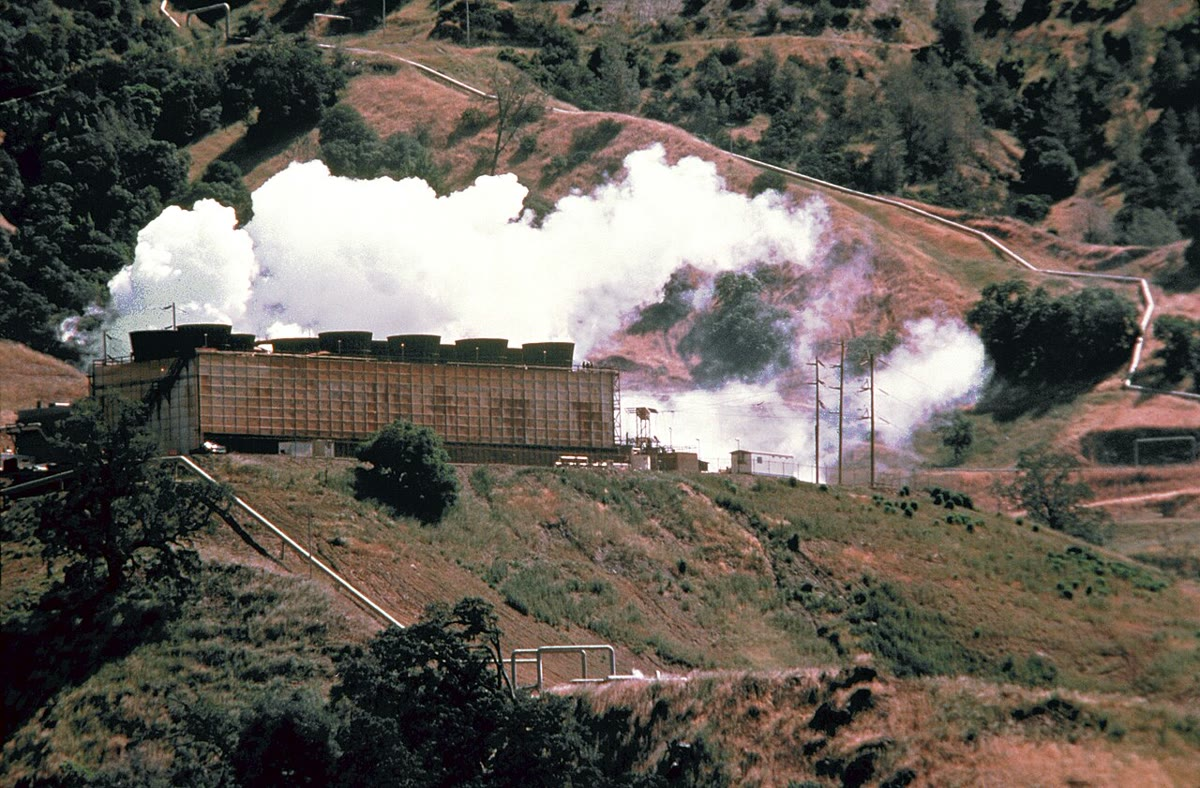
\includegraphics[width=\linewidth]{images/book4/b2-30-geyserville.jpg}
\end{minipage}
\par\smallskip{\small Kiri: \omterm{def:b2:energy-geology:geothermal}{sistem panas bumi} entalpi tinggi (skematis, tidak berskala): air
yang mengimbuh di tepi-tepinya (biru) terpanaskan di atas suatu intrusi dan naik (merah) melalui reservoir terekahkan
ke mata air panas; sumur-sumur menyadap reservoir itu. Kanan: pembangkit listrik panas bumi di dekat Geyserville,
California, pada 1982, dengan pipa-pipa uap di lereng bukit. Foto: Departemen Pertahanan AS
(domain publik).}
\end{omfigure}
% ledger: photo:b2-30-geyserville, usgs08g:egs

\begin{definition}[Seismisitas terinduksi]\label{def:b2:energy-geology:induced}
Yang disebut \emph{seismisitas terinduksi}\index{seismisitas terinduksi} adalah aktivitas gempa bumi yang disebabkan oleh kegiatan
manusia yang mengubah tegangan atau tekanan fluida pori di dalam kerak, paling sering
injeksi fluida ke dalam tanah.
\end{definition}

Mekanismenya adalah kriteria Coulomb dengan tekanan fluida pori: sesar tergelincir ketika tegangan geser
mencapai $\mu(\sigma_n - p)$, sehingga menaikkan $p$ membawa sesar yang sudah tertegang menuju keruntuhan
tanpa perubahan apa pun pada beban tektonik. Pada tahun 1960-an, fluida limbah yang diinjeksikan ke dalam batuan dasar
Prakambrium yang terekahkan di bawah Rocky Mountain Arsenal dekat Denver, pada kedalaman 3.7 sampai
\qty{7.0}{km}, memicu gempa bumi; gempa-gempa itu terbatas pada bagian reservoir tempat
tekanan telah naik lebih dari \qty{32}{bar} (\qty{3.2}{MPa}). Kenaikan tajam gempa bumi
di Oklahoma telah dikaitkan dengan pembuangan air limbah: empat sumur bervolume
tinggi dapat menjelaskan seperlima seismisitas Amerika Serikat bagian tengah, dengan memicu
gempa bumi yang berjarak lebih dari \qty{30}{km}. Stimulasi reservoir EGS menaikkan tekanan pori dengan
cara yang sama, secara sengaja.
% ledger: hb81:denver, keranen:oklahoma, usgs08g:egs

\section{Uranium}\label{sec:b2:energy-geology:uranium}

Dua \omterm{def:b2:ore-deposits:types}{tipe endapan bijih} menggambarkan cara uranium terkonsentrasi: satu pada ketidakselarasan purba,
yang lain di dalam batu pasir.

\begin{definition}[Endapan uranium terkait ketidakselarasan dan endapan uranium roll-front]\label{def:b2:energy-geology:uranium}
Yang disebut \emph{endapan uranium terkait ketidakselarasan}\index{endapan uranium terkait ketidakselarasan} adalah tubuh
pitchblende dan uraninit yang mengisi rekahan dan breksi di dalam pelit karbonan termetamorfosis dan
di dalam kuarsa arenit di atasnya, di bawah, di atas, atau memotong ketidakselarasan antara batuan \omterm{def:b2:precambrian-earth:eons}{Proterozoikum}
Awal dan Tengah di suatu \omterm{def:b2:basins-compared:types}{cekungan intrakratonik}. Yang disebut \emph{endapan uranium roll-front}\index{endapan uranium roll-front}
adalah tubuh mineral uranium berbentuk bulan sabit yang memotong perlapisan batu pasir
feldspatik atau tufaan pada batas antara tanah teroksidasi dan tereduksi, tempat
uranium diendapkan dalam lingkungan yang tereduksi secara lokal, di antara pirit.
\end{definition}

Endapan ketidakselarasan berada di dalam batuan berumur 1800 sampai \qty{1200}{\Ma}, yaitu pelit
termetamorfosis di bawah ketidakselarasan dan batu pasir tak termetamorfosis di atasnya; batuan induknya terkloritisasi, dan sekis grafitan yang
menyertai banyak di antaranya merupakan konduktor listrik yang kuat, sasaran survei elektromagnetik. Key
Lake, Cluff Lake, dan Rabbit Lake di Saskatchewan serta Jabiluka dan Ranger di Australia utara adalah
contohnya. Endapan roll-front lebih muda, kebanyakan Tersier: di dalam batu pasir yang dipasok oleh abu vulkanik felsik atau
granit, mineral besi teroksidasi terletak di arah atas kemiringan dari front itu dan mineral tereduksi di arah bawahnya, seperti di cekungan-cekungan
Wyoming dan Pesisir Teluk Texas.
% ledger: b1693:unconformity, b1693:sandstone

\begin{proposition}[Uranium-235 di masa lampau]\label{prop:b2:energy-geology:u235}
Misalkan $r_0$ adalah rasio atom $^{235}$U/$^{238}$U saat ini dan $\lambda_5$, $\lambda_8$ konstanta peluruhan
kedua isotop itu. Pada waktu $t$ yang lalu rasionya adalah
\begin{equation}
r(t) = r_0\,e^{(\lambda_5 - \lambda_8)\,t} ,
\label{eq:b2:energy-geology:u235}
\end{equation}
dan $^{235}$U menyusun fraksi $r/(1 + r)$ dari atom-atom uranium, dengan mengabaikan jejak
$^{234}$U.
\end{proposition}

\begin{proof}
Setiap isotop meluruh secara eksponensial: $N_5(\text{kini}) = N_5(t)\,e^{-\lambda_5 t}$ dan $N_8(\text{kini})
= N_8(t)\,e^{-\lambda_8 t}$. Dengan membagi keduanya, $r_0 = r(t)\,e^{-(\lambda_5 - \lambda_8)t}$.
\end{proof}

Dengan $\lambda_5 = \qty{9.8485e-10}{yr^{-1}}$, $\lambda_8 = \qty{1.55125e-10}{yr^{-1}}$ dan kelimpahan
saat ini \qty{0.7204}{\percent} dan \qty{99.2742}{\percent}, $r_0 = 0.0072567$; \qty{2.0}{\Ga}
yang lalu $r = 0.0381$ dan uranium alam memuat \qty{3.67}{\percent} $^{235}$U, lima kali bagiannya
saat ini.
% ledger: amherst:constants, iaea:isotopes
% values: r 0.038144, 3.6743 % (calc/ch30.py)

\begin{history}[Reaktor berumur dua miliar tahun]
Pada 1972, ilmuwan Prancis yang mengukur bijih uranium menemukan defisit $^{235}$U yang kecil tetapi berarti,
yang mereka telusuri sampai ke tambang Oklo di Gabon. Di sana, kantong-kantong batuan memuat sampai
\qty{65}{\percent} uranium dengan bagian $^{235}$U serendah separuh bagian normal, dan neodimium
yang miskin isotop primordialnya $^{142}$Nd tetapi kaya isotop 143 sampai 150 yang dihasilkan
fisi: reaksi berantai telah berlangsung di dalam bijih itu sekitar dua miliar tahun yang lalu, pada sekitar \qty{300}{bar}
dan 400 sampai \qty{500}{\celsius}. Enam belas reaktor alam semacam itu diketahui di Oklo dan di
Bangombé yang berdekatan, satu-satunya dua endapan di dunia tempat reaktor itu ditemukan; bahan organik telah membantu
memekatkan uranium, dan uranium oksida telah menahan sebagian besar aktinida dan
produk fisi yang tidak mudah menguap di tempatnya sejak saat itu.
\end{history}
% ledger: oklo:curtis, oklo:cowan, oklo:gl96, oklo:nagy

\section{Penyimpanan geologis karbon dioksida}\label{sec:b2:energy-geology:ccs}

\begin{definition}[Penyimpanan \ce{CO2} geologis, mekanisme pemerangkapan, faktor efisiensi penyimpanan]\label{def:b2:energy-geology:ccs}
Yang disebut \emph{penyimpanan \ce{CO2} geologis}\index{penyimpanan CO$_2$ geologis} adalah injeksi karbon
dioksida ke dalam formasi batuan berpori jauh di bawah tanah, yaitu reservoir minyak dan gas yang telah terkuras, formasi salin
dalam, atau lapisan batu bara, untuk ditahan dalam waktu lama. Yang disebut \emph{mekanisme pemerangkapan
\ce{CO2}}\index{mekanisme pemerangkapan CO$_2$} yang menahannya adalah pemerangkapan struktural (dan stratigrafis)
di bawah batuan penutup; pemerangkapan residual, sebagai fase tak bergerak yang ditahan di dalam pori oleh gaya
kapiler; pemerangkapan kelarutan, dengan pelarutan di dalam air formasi; pemerangkapan mineral, dengan reaksi
dengan mineral menjadi karbonat; dan, di dalam batu bara dan serpih, adsorpsi pada bahan organik.
Yang disebut \emph{faktor efisiensi penyimpanan}\index{faktor efisiensi penyimpanan} $E$ suatu formasi adalah fraksi volume porinya yang diharapkan
dapat diisi oleh \ce{CO2} yang diinjeksikan.
\end{definition}
% ledger: srccs:retention, netl08:saline

Karbon dioksida berupa gas di permukaan, tetapi titik kritisnya terletak pada \qty{31.0}{\celsius} dan
\qty{7.38}{MPa}. Di sepanjang geoterm \qty{25}{\celsius\per\km} dari \qty{15}{\celsius} di bawah
tekanan hidrostatik, suhu melewati nilai kritisnya pada \qty{641}{m} dan tekanan pada
\qty{742}{m}; densitas \ce{CO2} murni melonjak dari \qty{234}{kg.m^{-3}} pada \qty{700}{m} menjadi
\qty{583}{kg.m^{-3}} pada \qty{900}{m}, lalu mendatar di dekat 670 sampai \qty{700}{kg.m^{-3}} di bawah
\qty{1.5}{km}. Satu ton menempati \qty{534}{m^3} di permukaan dan \qty{1.6}{m^3} pada \qty{1000}{m},
330 kali lebih kecil; itulah sebabnya penilaian penyimpanan hanya mempertimbangkan formasi yang lebih dalam dari
\qty{800}{m}.
% ledger: nist:co2-critical, data:b4-co2-density, srccs:density, netl08:saline
% values: z_tc 641.2 m, z_pc 742.2 m; volume ratio 331.9 (figdata co2_density.py numbers)

\begin{omfigure}
\centering
\begin{minipage}[b]{0.49\linewidth}\centering
\begin{tikzpicture}
\begin{axis}[omrecord, width=0.95\linewidth, height=5.2cm, xmin=0, xmax=750, ymin=0, ymax=3,
  y dir=reverse, xlabel={densitas \ce{CO2} (\unit{kg.m^{-3}})}, ylabel={kedalaman (km)},
  tick label style={font=\scriptsize}, label style={font=\small}]
% computed in figdata/bachelor-2/co2_density.py part profile; ledger: data:b4-co2-density
\addplot[black!45, densely dashed] coordinates {(0,0.742) (750,0.742)};
\node[font=\tiny, text=black!60, anchor=south east] at (axis cs:745,0.73) {tekanan kritis};
\addplot[omDef, line width=1.1pt, mark=*, mark size=0.9pt] table[x=rho, y expr=\thisrow{depth_m}/1000] {figdata/out/bachelor-2-co2_density-profile.dat};
\end{axis}
\end{tikzpicture}
\end{minipage}\hfill
\begin{minipage}[b]{0.49\linewidth}\centering
\begin{tikzpicture}
\begin{axis}[width=0.95\linewidth, height=5.2cm, xmin=0, xmax=4, ymin=0, ymax=100,
  axis x line=bottom, axis y line=left, axis line style={-}, axis on top,
  xlabel={waktu setelah injeksi (tahun)}, ylabel={bagian \ce{CO2} yang tersimpan},
  xtick={0,1,2,3,4}, xticklabels={1,10,100,1000,$10^4$}, ytick=\empty,
  tick label style={font=\scriptsize}, label style={font=\small}]
% schematic, after IPCC SRCCS (2005) Figure 5.9; ledger: srccs:trapping
% bands from the bottom: mineral, solubility, residual, structural (cumulative tops 0/0/1/5/15,
% 2/8/21/40/60, 10/30/56/80/90, 100)
\fill[omLithLime!60!black] (axis cs:0,0) -- (axis cs:1,0) -- (axis cs:2,1) -- (axis cs:3,5) -- (axis cs:4,15) -- (axis cs:4,0) -- cycle;
\fill[omDef!40] (axis cs:0,0) -- (axis cs:1,0) -- (axis cs:2,1) -- (axis cs:3,5) -- (axis cs:4,15) -- (axis cs:4,60) -- (axis cs:3,40) -- (axis cs:2,21) -- (axis cs:1,8) -- (axis cs:0,2) -- cycle;
\fill[omProp!40] (axis cs:0,2) -- (axis cs:1,8) -- (axis cs:2,21) -- (axis cs:3,40) -- (axis cs:4,60) -- (axis cs:4,90) -- (axis cs:3,80) -- (axis cs:2,56) -- (axis cs:1,30) -- (axis cs:0,10) -- cycle;
\fill[black!15] (axis cs:0,10) -- (axis cs:1,30) -- (axis cs:2,56) -- (axis cs:3,80) -- (axis cs:4,90) -- (axis cs:4,100) -- (axis cs:0,100) -- cycle;
\node[font=\scriptsize] at (axis cs:1.1,72) {struktural};
\node[font=\scriptsize] at (axis cs:2.1,38) {residual};
\node[font=\scriptsize] at (axis cs:3.1,22) {kelarutan};
\node[font=\scriptsize, text=white, anchor=south east] at (axis cs:3.98,0.5) {mineral};
\end{axis}
\end{tikzpicture}
\end{minipage}
\par\smallskip{\small Kiri: densitas \ce{CO2} murni terhadap kedalaman di sepanjang geoterm
\qty{25}{\celsius\per\km} dari \qty{15}{\celsius}, di bawah tekanan hidrostatik. Data: NIST Chemistry
WebBook (persamaan keadaan Span--Wagner), pada kondisi Laporan Khusus IPCC tentang Penangkapan
dan Penyimpanan Karbon Dioksida (2005). Kanan: cara mekanisme-mekanisme pemerangkapan membagi \ce{CO2} yang tersimpan
seiring waktu (skematis, menurut laporan yang sama): pemerangkapan oleh batuan penutup digantikan oleh bentuk residual,
terlarut, dan mineral, yang kurang mudah bergerak.}
\end{omfigure}

\begin{proposition}[Kapasitas penyimpanan suatu formasi]\label{prop:b2:energy-geology:capacity}
Suatu formasi dengan luas $A$, tebal $h$, dan porositas $\phi$, tempat \ce{CO2} memiliki densitas $\rho$
dan \omterm{def:b2:energy-geology:ccs}{faktor efisiensi penyimpanannya} $E$, dapat menyimpan massa
\begin{equation}
M = A\,h\,\phi\,\rho\,E .
\label{eq:b2:energy-geology:capacity}
\end{equation}
Untuk lapangan minyak terkuras yang telah memproduksi volume tangki stok $N_p$, penggantian minyak yang diproduksi
volume demi volume memberikan $M = \rho\,N_p\,B_o$.
\end{proposition}

\begin{proof}
Volume porinya adalah $Ah\phi$, yang sebagian $E$-nya diisi \ce{CO2}, dengan densitas $\rho$. Di lapangan
minyak, minyak yang diproduksi menempati $N_pB_o$ di dalam reservoir, volume yang diambil alih oleh \ce{CO2}.
\end{proof}

Untuk formasi salin dalam, simulasi memberikan $E$ antara 1 dan \qty{4}{\percent} volume pori
dalam rentang kepercayaan 15 sampai 85 persen, dengan median di dekat \qty{2}{\percent}: sebagian besar ruang
pori tidak pernah tercapai, atau tetap berisi airnya. Formasi seluas \qty{1000}{km^2}, setebal \qty{50}{m}, dan
berporositas 0.20 pada \qty{2000}{m} ($\rho = \qty{686}{kg.m^{-3}}$) menyimpan \qty{137}{Mt} pada $E =
\qty{2}{\percent}$.
% ledger: netl08:saline, data:b4-co2-density
% values: 1e9*50*0.2*686*0.02 = 1.372e11 kg (calc/ch30.py)

Setelah diinjeksikan, \ce{CO2} naik ke bawah batuan penutup dan menyebar. Di belakang plume yang bermigrasi, gaya
kapiler menahan saturasi residual yang dapat mencapai 15 sampai \qty{25}{\percent} ruang pori;
pelarutan menyerap 20 sampai \qty{60}{kg} \ce{CO2} per meter kubik air formasi, dan di dalam
formasi yang alirannya lambat sampai \qty{30}{\percent} \ce{CO2} yang diinjeksikan larut dalam puluhan
tahun. Pemerangkapan kelarutan mendominasi selama puluhan sampai ratusan tahun, bentuk ionik selama ratusan sampai
ribuan tahun, pemerangkapan mineral selama ribuan sampai jutaan tahun: reaksi dengan mineral karbonat berlangsung beberapa hari,
dengan silikat ratusan sampai ribuan tahun. Penyimpanan menjadi makin aman seiring umurnya, dan di
lokasi yang dipilih dan dikelola dengan baik, tertahannya \qty{99}{\percent} atau lebih \ce{CO2} selama
1000 tahun dinilai mungkin.
% ledger: srccs:trapping, srccs:retention

\begin{dated}{2005}
Di Sleipner, di Laut Utara sekitar \qty{250}{km} lepas pantai Norwegia, \ce{CO2} yang dipisahkan dari
gas alam lapangan itu, sekitar \qty{9}{\percent} darinya, telah diinjeksikan sejak Oktober 1996 ke dalam
formasi Utsira, batu pasir salin tak terkonsolidasi 800 sampai \qty{1000}{m} di bawah dasar laut,
dengan laju sekitar \qty{1}{Mt} setahun. Pada awal 2005 lebih dari \qty{7}{Mt} telah tersimpan, dari \qty{20}{Mt}
yang direncanakan sepanjang umur proyek. Survei seismik berulang mencitrakan plume itu, yang jejaknya saat itu
sekitar \qty{5}{km^2}, dan menunjukkan bahwa batuan tudung di atasnya menyegelnya.
\end{dated}
% ledger: srccs:sleipner

\begin{inthefield}[Membaca sumur selagi dibor]
\centering
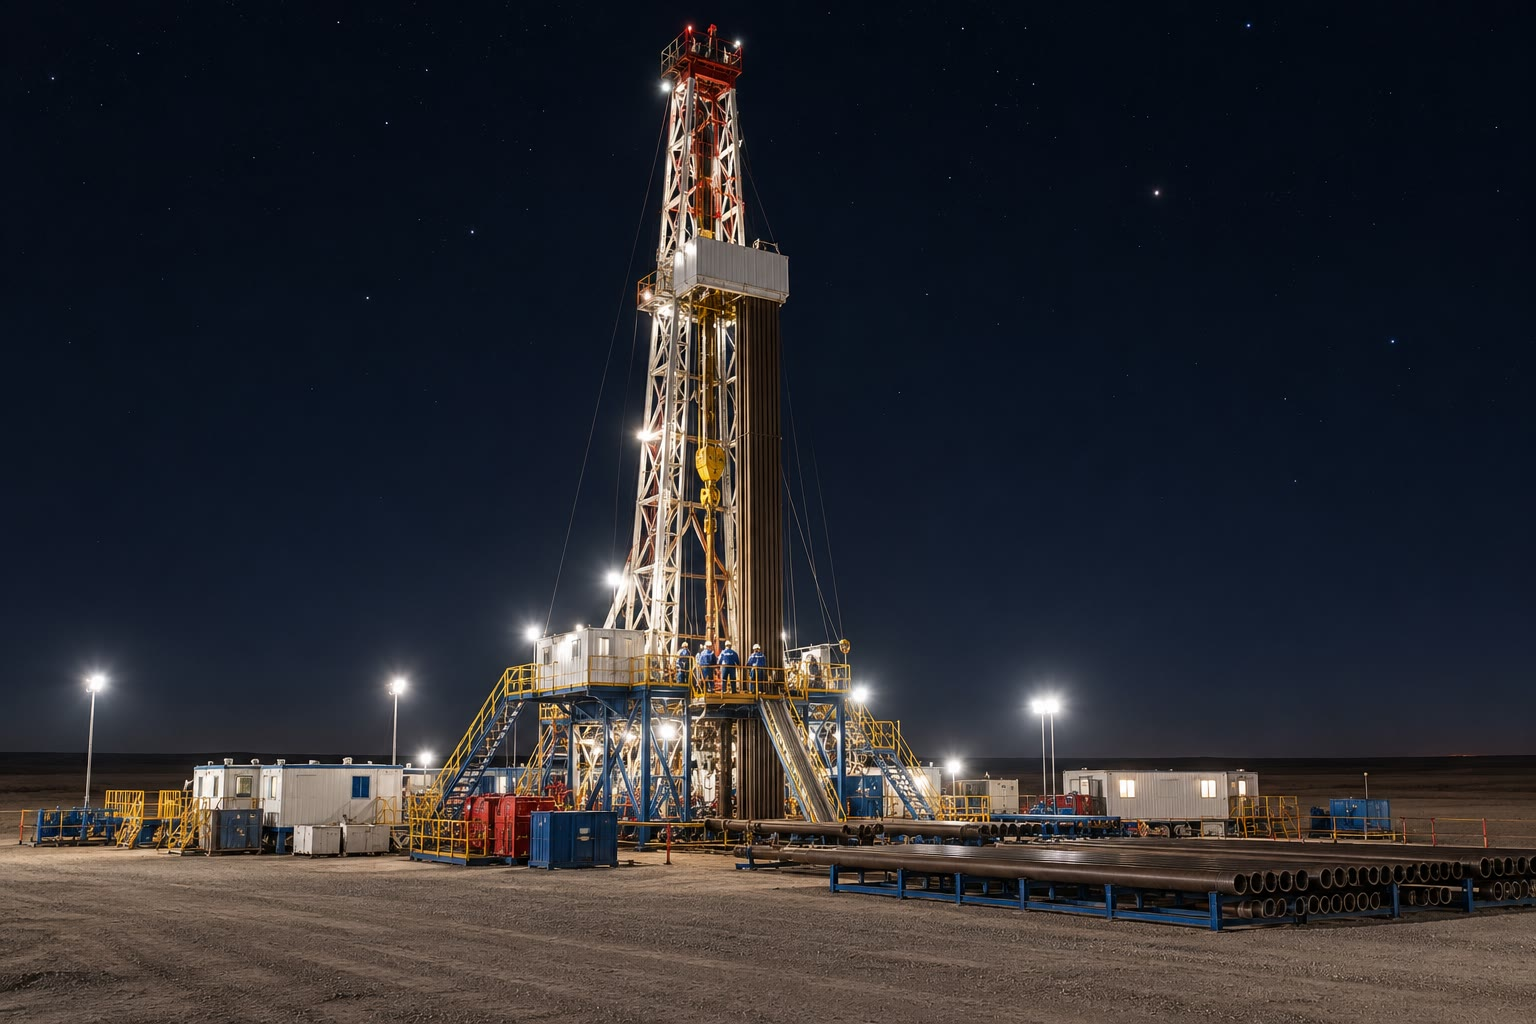
\includegraphics[width=0.56\linewidth]{images/book4/ai/b2-rig-night.jpg}
\par\smallskip{\small Rig pengeboran darat pada malam hari (ilustrasi buatan AI).}
\par\medskip\raggedright
Ketika satu bagian sumur selesai, para ahli geofisika menurunkan alat-alat dengan kabel dan merekam terhadap
kedalaman sifat-sifat batuan di sekitar lubang. Satu alat merekam radioaktivitas alaminya, rendah di
batu pasir dan lebih tinggi di serpih; alat lain merekam densitas totalnya, yang darinya porositas diperoleh sebagai
(densitas butir $-$ densitas total)/(densitas butir $-$ densitas fluida), dengan \qty{2.65}{g/cm^3} untuk
butir kuarsa dan sekitar \qty{1}{g/cm^3} untuk air. Bila dibaca bersama, log-log lubang bor ini memberikan
ketebalan reservoir bersih dan porositas yang masuk ke dalam rumus-rumus volumetrik bab ini.
\end{inthefield}
% ledger: keys:gamma, keys:density-porosity

\section*{Latihan}\label{sec:b2:energy-geology:exercises}

Data untuk latihan, kecuali dinyatakan lain: $R = \qty{8.314}{J.mol^{-1}.K^{-1}}$; satu juta
tahun adalah \qty{3.156e13}{s}; kerogen Green River $A = \qty{9.21e13}{s^{-1}}$, $E/R = \qty{26800}{K}$;
massa atom C 12.011, H 1.008, O 15.999; densitas \ce{CO2} di sepanjang profil pada gambar:
\qty{1.872}{kg.m^{-3}} di permukaan, 583 pada \qty{900}{m}, 621 pada \qty{1000}{m}, 686 pada
\qty{2000}{m}. Bulatkan sampai tiga angka penting.
% ledger: codata:R, fp14:gr-daem, data:b4-co2-density

\begin{exercise}[$\star$]\label{exo:b2:energy-geology:1}
(a) Empat kerogen belum matang memiliki H/C atom 1.58, 0.95, 1.24, dan 1.12. Tentukan tipe masing-masing dan sebutkan
mana yang terutama akan menghasilkan gas. (b) Periksa rasio H/C dan O/C rumus
C$_{100}$H$_{150}$N$_3$O$_8$S. (c) Tentukan keduanya dari komposisi massa C \qty{77.4}{\percent}, H
\qty{9.8}{\percent}, O \qty{8.2}{\percent}.
\end{exercise}

\begin{exercise}[$\star$]\label{exo:b2:energy-geology:2}
(a) Lima sampel batuan sumber tipe~II memiliki $R_o$ = 0.45, 0.68, 1.1, 1.6, dan \qty{2.5}{\percent}.
Uraikan keadaan masing-masing terkait minyak dan gas. (b) Apakah kerogen tipe~III pada $R_o =
\qty{0.68}{\percent}$ sedang menghasilkan metana? (c) Fraksi terkonversi $F$ Easy\%Ro berapakah yang bersesuaian dengan
$R_o = 0.6$ dan \qty{1.3}{\percent}?
\end{exercise}

\begin{exercise}[$\star$]\label{exo:b2:energy-geology:3}
Suatu perangkap meliputi \qty{6}{km^2}; reservoirnya memiliki ketebalan bersih \qty{25}{m}, porositas 0.18, dan saturasi
air 0.30, dan $B_o = 1.25$. (a) Tentukan volume minyak di dalam reservoir dan STOIIP-nya. (b) Tentukan
volume yang diproduksi untuk \omterm{def:b2:energy-geology:volumetrics}{faktor perolehan} 0.30 dan 0.40.
\end{exercise}

\begin{exercise}[$\star$]\label{exo:b2:energy-geology:4}
Akuifer batu pasir setebal \qty{200}{m} di bawah \qty{10}{km^2} bersuhu \qty{75}{\celsius}. (a) Tentukan
\omterm{def:b2:energy-geology:geothermal}{panas di tempatnya} di atas \qty{15}{\celsius}, dengan $C = \qty{2.5}{MJ.m^{-3}.K^{-1}}$. (b) Termasuk kelas
entalpi manakah akuifer itu? (c) Tentukan daya termal rata-rata selama 30 tahun untuk $R_g = 0.25$.
\end{exercise}

\begin{exercise}[$\star\star$]\label{exo:b2:energy-geology:5}
(a) Tentukan energi aktivasi yang membuat laju Arrhenius berlipat dua antara 100 dan
\qty{110}{\celsius}. (b) Dengan faktor berapa laju reaksi Green River bertambah dalam selang
yang sama? (c) Manakah dari kedua aturan itu yang memberi bobot lebih besar pada waktu yang dilewatkan batuan pada suhu rendah,
dan apa implikasinya bagi TTI yang dihitung untuk batuan sumber tipe~I?
\end{exercise}

\begin{exercise}[$\star\star$]\label{exo:b2:energy-geology:6}
(a) Tunjukkan dari \eqref{eq:b2:energy-geology:maturation} bahwa suhu konversi separuh memenuhi
$T = (E/R)\big/\ln\bigl[A T^2/(\beta\,(E/R)\ln 2)\bigr]$, dan selesaikan dengan iterasi untuk kerogen Green
River yang dipanaskan dengan laju \qty{1}{\celsius\per\Ma} dan \qty{10}{K} per menit. (b) Bandingkan
selisihnya dengan taksiran $(RT^2/E)\ln(\beta_2/\beta_1)$ yang diambil pada suhu yang lebih rendah, dan
jelaskan ketidaksesuaiannya.
\end{exercise}

\begin{exercise}[$\star\star$]\label{exo:b2:energy-geology:7}
Dengan \eqref{eq:b2:energy-geology:u235} dan data dalam teks: (a) tentukan bagian $^{235}$U dalam
uranium alam \qty{2.0}{\Ga} dan \qty{1.8}{\Ga} yang lalu; (b) kapan bagian itu \qty{3.00}{\percent}?
(c) Bijih Oklo memuat $^{235}$U serendah separuh bagian normal saat ini. Dengan mengabaikan $^{238}$U
yang terpakai, berapa fraksi $^{235}$U yang ada pada saat reaksi-reaksi itu yang telah mengalami fisi, dan
mengapa peluruhan sesudahnya tidak mengubah jawabannya?
\end{exercise}

\begin{exercise}[$\star\star$]\label{exo:b2:energy-geology:8}
(a) Tentukan volume \qty{1}{Mt} \ce{CO2} di permukaan, pada \qty{1000}{m}, dan pada
\qty{2000}{m}. (b) Di Sleipner lebih dari \qty{7}{Mt} telah diinjeksikan pada 2005, pada sekitar
\qty{900}{m}, ke dalam plume dengan jejak \qty{5}{km^2}. Dengan porositas 0.35 dan saturasi \ce{CO2}
0.30 di dalam plume, tentukan volume batuan yang ditempatinya dan tebal rata-ratanya.
\end{exercise}

\begin{exercise}[$\star\star$]\label{exo:b2:energy-geology:9}
Suatu reservoir entalpi tinggi berukuran $3 \times 2 \times \qty{1.5}{km}$ pada \qty{250}{\celsius}, dengan
$C = \qty{2.6}{MJ.m^{-3}.K^{-1}}$. (a) Tentukan \omterm{def:b2:energy-geology:geothermal}{panas di tempatnya} di atas \qty{15}{\celsius}. (b) Tentukan
daya termal rata-rata selama 30 tahun untuk $R_g = 0.1$ dan $0.25$. (c) Lapangannya meliputi \qty{6}{km^2};
dengan 10 sampai \qty{20}{MW} listrik per kilometer persegi, berapa fraksi daya termal pada
$R_g = 0.1$ yang menjadi listrik?
\end{exercise}

\begin{exercise}[$\star\star\star$]\label{exo:b2:energy-geology:10}
Suatu sesar pada kedalaman sekitar \qty{4}{km} menanggung tegangan normal \qty{80}{MPa} dan tegangan geser
\qty{22}{MPa}; koefisien gesekannya 0.6 dan tekanan porinya hidrostatik,
\qty{39}{MPa}. (a) Apakah sesar itu stabil? Tentukan kenaikan tekanan pori yang membawanya ke keruntuhan, dalam
megapascal dan dalam bar, dan bandingkan dengan ambang Denver. (b) Hal yang sama jika tegangan gesernya
\qty{24}{MPa}. (c) Jelaskan mengapa gempa bumi dapat terpicu berkilometer-kilometer jauhnya dari sumur injeksi,
dan bertahun-tahun setelah injeksi dimulai.
\end{exercise}

\begin{exercise}[$\star\star\star$]\label{exo:b2:energy-geology:11}
(a) Dari pendekatan dalam \eqref{eq:b2:energy-geology:maturation}, tunjukkan bahwa pada laju
pemanasan tetap rasio transformasi naik dari \qty{10}{\percent} menjadi \qty{90}{\percent} dalam selang
suhu $\Delta T \approx \bigl[\ln\ln 10 - \ln\ln(10/9)\bigr]\,RT^2/E$. (b) Hitunglah nilainya
untuk kerogen Green River pada \qty{1}{\celsius\per\Ma}. (c) Bandingkan dengan kurva garis utuh pada
gambar dan jelaskan perbedaannya.
\end{exercise}

\begin{exercise}[$\star\star\star$]\label{exo:b2:energy-geology:12}
Sleipner akan menyimpan \qty{20}{Mt} \ce{CO2}. (a) Tentukan volume air formasi yang diperlukan untuk
melarutkan semuanya, pada 20 dan pada \qty{60}{kg.m^{-3}}. (b) Tentukan volumenya sebagai fase bebas pada
\qty{1000}{m}. (c) Dengan $E = \qty{2}{\percent}$, tentukan volume pori formasi yang diperlukan, dan
luas formasi setebal \qty{50}{m} dengan porositas 0.30.
\end{exercise}
% ledger: srccs:trapping, srccs:sleipner, hb81:denver

\begin{problem}[{Soal akhir pekan --- Satu cekungan, dua kegunaan}]\label{pb:b2:energy-geology:1}
Di suatu cekungan rekaan, batuan sumber tipe~I diendapkan pada \qty{120}{\Ma} di permukaan.
Sedimen kemudian terakumulasi dengan laju \qty{60}{m} per juta tahun sampai \qty{70}{\Ma}, dan \qty{30}{m}
per juta tahun sejak itu. Permukaan bersuhu \qty{15}{\celsius} dan geotermnya tetap,
\qty{25}{\celsius\per\km}. Kerogennya memiliki kinetika Green River dalam teks (energi tunggal).
Dapurnya, yaitu bagian batuan sumber yang matang, meliputi \qty{400}{km^2}, setebal \qty{50}{m},
berdensitas \qty{2400}{kg.m^{-3}}, dan dapat menghasilkan \qty{30}{kg} minyak per ton batuan pada konversi
penuh; minyaknya berdensitas permukaan \qty{850}{kg.m^{-3}}. Minyak itu mengisi perangkap seluas
\qty{12}{km^2} yang reservoirnya, berpusat pada \qty{2000}{m}, memiliki ketebalan bersih \qty{40}{m},
porositas 0.22, dan saturasi air 0.25, dengan $B_o = 1.30$. Gunakan data latihan; bulatkan sampai
tiga angka penting.

\noindent\textbf{Bagian I --- Penimbunan dan indeks waktu--suhu.}
\begin{enumerate}
  \item Tentukan kedalaman dan suhu batuan sumber pada \qty{70}{\Ma} dan saat ini.
  \item Tentukan laju pemanasannya dalam setiap fase.
  \item Tentukan waktu yang dilewatkannya dalam setiap selang \qty{10}{\celsius}, dari \qty{15}{\celsius} sampai
        suhunya saat ini.
  \item Hitunglah TTI-nya saat ini (metode dalam teks).
  \item Kapan, pada suhu berapa, dan pada kedalaman berapa batuan itu melewati TTI 15?
  \item Hal yang sama untuk 75 dan 160.
  \item Menurut TTI, apakah batuan sumber itu masih menghasilkan minyak?
\end{enumerate}

\noindent\textbf{Bagian II --- Konversi menurut kinetika.}
\begin{enumerate}[resume]
  \item Tentukan konstanta laju pada \qty{90}{\celsius} dan tunjukkan bahwa kerogen yang dapat terkonversi
        sebelum \qty{70}{\Ma} kurang dari \qty{0.2}{\percent}.
  \item Dengan \eqref{eq:b2:energy-geology:maturation} dan laju pemanasan fase kedua,
        tentukan fraksi yang belum terkonversi dan rasio transformasi saat ini.
  \item Tentukan suhu konversi separuh pada laju pemanasan ini (latihan~\ref{exo:b2:energy-geology:6}).
  \item Kapan suhu itu tercapai?
  \item Bandingkan dengan waktu puncak pembentukan minyak menurut TTI, dan jelaskan perbedaannya.
  \item Apakah kerogen tipe~II dengan energi aktivasi rata-rata yang lebih rendah akan terkonversi lebih awal atau lebih lambat?
\end{enumerate}

\noindent\textbf{Bagian III --- Minyak yang terbentuk, di tempat, dan yang dapat diperoleh.}
\begin{enumerate}[resume]
  \item Dengan rasio transformasi 0.92, tentukan massa minyak yang terbentuk di dapur.
  \item Tentukan volumenya di permukaan.
  \item Tentukan STOIIP perangkap itu.
  \item Berapa fraksi minyak yang terbentuk yang ditampung perangkap? Pakailah \qty{1.56e9}{m^3} untuk (15).
  \item Tentukan minyak yang diproduksi untuk \omterm{def:b2:energy-geology:volumetrics}{faktor perolehan} 0.35.
  \item Mengapa \omterm{def:b2:energy-geology:volumetrics}{faktor perolehan} jauh lebih kecil daripada satu, dan apa yang akan diubah oleh injeksi \ce{CO2}?
\end{enumerate}

\noindent\textbf{Bagian IV --- Lapangan terkuras sebagai penyimpan \ce{CO2}.}
\begin{enumerate}[resume]
  \item Tentukan suhu dan tekanan hidrostatik reservoir. Apakah \ce{CO2} yang diinjeksikan
        superkritis di sana? Bacalah densitasnya pada gambar.
  \item Dengan $N_p = \qty{2.13e7}{m^3}$, tentukan volume reservoir yang dibebaskan oleh produksi.
  \item Nyatakan volume itu sebagai \omterm{def:b2:energy-geology:ccs}{faktor efisiensi penyimpanan} volume pori perangkap, dan bandingkan dengan
        formasi salin.
  \item Suatu formasi salin di bawah lapangan itu meliputi \qty{600}{km^2}, setebal \qty{80}{m},
        berporositas 0.20, dengan \ce{CO2} pada \qty{691}{kg.m^{-3}}. Tentukan kapasitasnya pada $E =
        \qty{2}{\percent}$.
  \item Berapa tahun injeksi dengan laju Sleipner akan mengisinya?
  \item Dengan $\rho = \qty{686}{kg.m^{-3}}$ dan volume yang dibebaskan dibulatkan menjadi \qty{2.77e7}{m^3}, tentukan
        kapasitas penyimpanan \ce{CO2} reservoir terkuras itu, dalam megaton.
\end{enumerate}
\end{problem}
% ledger: fp14:gr-daem, waples80:tti, hamm14:tti-table, netl08:oilgas, netl08:saline, data:b4-co2-density, nist:co2-critical, srccs:sleipner
